\section{Part 2: Calculus}

\subsection{Derivatives: Polynomials, Power Functions, Product and Chain Rule, Multivariate Calculus}

\begin{frame}{Intuition}
    \textbf{Geometrically}: The derivative is the tangent line to the curve at the point $(x0, y0)$
    is a line passing through $(x0, y0)$ and `flat against' the curve

    \begin{center}
        \includesvg[width=0.3\textwidth]{fig/tangent_to_a_curve}
    \end{center}

    \textbf{Intuition}: The derivative measures the sensitivity to change of the function value
    (output value) with respect to a change in its argument (input value)\\[5mm]

\end{frame}

\begin{frame}{Definition}
    Roughly speaking, a function $f(x)$ is differentiable at a point $a$ of its domain,
    if the limit
    $$L=\lim_{h \to 0}\frac{f(a+h)-f(a)}h$$
    exists.

    \begin{boxed}
        If the limit $L$ exists, then this limit is called the \emph{derivative} of $f$ at $a$,
        and denoted $$f'(a) \quad \text{or} \quad \frac{df}{dx}(a)$$
    \end{boxed}
\end{frame}



\begin{frame}{Derivatives of polynomials}
    There's just four simple facts which suffice to take the derivative
    of any polynomial plussomewhat more general things.

    First, there is the rule for taking the derivative of a \emph{power function}
    $f(x)=x^n$:
    $${d\over dx}x^n=n\,x^{n-1}$$

    Second, a special case of the rule above, the derivative of any constant $c$ is zero:
    $${d\over dx}\,c=0$$

    Third, for any function $f(x)$, multiplicative constants do not affect the result,
    $${d\over dx}\,c f=c \,{d\over dx}\,f$$

    Fourth, for any two functions $f(x)$ and  $g(x)$, the derivative of the sum
    is the sum of the derivatives:
    $${d\over dx}(f+g)={d\over dx}f+{d\over dx}g$$
\end{frame}

\begin{frame}
    Putting these four things together, we can write general formulas like
    $${d\over dx}(ax^m+bx^n+cx^p)=a\,m\,x^{m-1}+b\,n\,x^{n-1}+c\,p\,x^{p-1}$$
    and so on, with any number of summands.

    As a refresher, here are some examples:

    $${d\over dx}5x^3=15x^2$$
    $${d\over dx}(3x^7+5x^3-11)=21x^6+15x^2$$
    $${d\over dx}(2-3x^2-2x^3)=-6x-6x^2$$
    $${d\over dx}(-x^4+2x^5+ 1)=-4x^3+10x^4$$
\end{frame}

\begin{frame}{More general power functions}
    Remember some of the other possibilities for the exponential notation $x^n$. For example
    $$x^{{1\over 2}}=\sqrt{x}$$
    $$x^{-1}={1\over x}$$
    $$x^{-{1\over 2}}={ 1 \over \sqrt{x }}$$
    and so on.

    Good news: Above rule for taking
    the derivative of powers of $x$ is still correct here, even for
    exponents which are negative or fractions or even real numbers:

    $$ {d\over dx}x^r=r\,x^{r-1}$$
\end{frame}

\begin{frame}
    Thus, in particular,
    $${d\over dx}\sqrt{x}=
        {d\over dx}x^{{1\over 2}}={1\over 2}x^{-{1\over 2}}$$
    $${d\over dx}{1\over x}={d\over dx}x^{-1}=-1\cdot
        x^{-2}={-1\over x^2}$$

    When combined with the sum rule from above, we have the
    obvious possibilities:

    $${d\over dx}(3x^2-7\sqrt{x}+{5\over x^2})=
        {d\over dx}(3x^2-7x^{{1\over 2}}+5x^{-2})=
        6x-{7\over 2}x^{-{1\over 2}}-10x^{-3}$$

    \begin{boxed}
        Expressing square roots, cube roots, inverses,
        etc., in terms of exponents often simplifies
        the rearranging of algebraic expressions
    \end{boxed}

\end{frame}

\begin{frame}{Quotient rule}
    \begin{boxed}
        \textbf{Quotient rule}:
        Given two differentiable functions $f(x)$ and $g(x)$, the derivative of the
        ratio of the two is given by:
        $${d\over dx}{f\over g}={f'g-g'f\over g^2}$$
    \end{boxed}

    Example: For $f(x) = x-1$ and $g(x) = x-2$ we get
    $${d\over dx}{x-1\over x-2}=
        {(x-1)'(x-2)-(x-1)(x-2)'\over (x-2)^2}=
        {1\cdot(x-2)-(x-1)\cdot 1\over (x-2)^2}$$
    $$=
        {(x-2)-(x-1)\over (x-2)^2}=
        {-1\over (x-2)^2}$$
\end{frame}

\begin{frame}
    Special case of the quotient rule: Applying the quotient rule to the
    expression $1 / g(x)$ yields
    \begin{boxed}
        \textbf{Reciprocal rule}:
        $$\frac{d}{dx}\frac{1}{g(x)}=-\frac{g'(x)}{g(x)^2}$$
    \end{boxed}

    Because
    $$\frac{d}{dx}\frac{1}{g(x)}=\frac{0 \cdot g(x) - 1 \cdot g'(x)}{g(x)^2}=\frac{-g'(x)}{g(x)^2}$$
\end{frame}

\begin{frame}{Product rule}
    We have:
    \begin{boxed}
        \textbf{Product rule}:
        $${d\over dx}(fg)=f'g+fg'$$
    \end{boxed}
    Note the this rule behaves differently from the simple rule for sums above

    Example: Differentiate $f(x) = x^2 \sin x$. We get $f'(x) = 2 x \sin x + x^2 \cos x$

    Note: ``constant multiple rule'' is a special case: $(c f(x))' = c f'(x)$ since ${d \over dx} c = 0$
\end{frame}

\easterchallenge{Find the derivative of the sigmoid function
    $$\sigma(x) = \frac{1}{1 + e^{-x}}$$
    and express it using the sigmoid function itself.
    Hint: Remember that in general $\frac{1}{1 + a} = \frac{1 + a - 1}{1 + a} = 1 - \frac{1}{1 + a}$
}{
    $$\frac{d}{\d \sigma} \frac{1}{1 + e^{-x}} = \ldots
        = \frac{1}{1 + e^{-x}} \frac{e^{-x}}{1 + e^{-x}}
        = \frac{1}{1 + e^{-x}} \frac{1 + e^{-x} - 1}{1 + e^{-x} }
        = \frac{1}{1 + e^{-x}}\left( 1 - \frac{1}{1 + e^{-x} }\right)
        = \sigma(x) \, (1 - \sigma(x))
    $$
}

\begin{frame}{Chain rule}
    Function composition operator ``$\circ$'':\\
    Operator that takes two functions $f$ and $g$ and produces a function $h = g \circ f$
    such that $h(x) = g(f(x))$. In other words, $g$ is applied to the result of $f(x)$.\\[5mm]

    The chain rule states how the derivative of the composition of two
    differentiable functions $f$ and $g$ behaves:
    \begin{boxed}
        \textbf{Chain rule}:
        $$h'=(f\circ g)'=(f'\circ g)\cdot g'$$
        \center{or less formally}
        $${d\over dx} f(g(x))=f'(g(x))\cdot g'(x)$$
    \end{boxed}

    Note that the chain rule is a core utility in machine learning, e.g. forming the base of
    how neural networks are learning, among countless other uses.
\end{frame}

\begin{frame}
    Use of chain rule is often straightforward. Just be clear what $f(x)$ and what $g(x)$ are.

    Here are some examples.

    Example 1:
    $${d\over dx}(1+x^2)^{100}=f'(g(x))\cdot g'(x)=100\,g^{99}(x)\cdot 2x=
        100\,(1+x^2)^{99}\cdot 2x$$

    Example 2:
    $${d\over dx}\sqrt{3x+2}={d\over dx}(3x+2)^{1/2}=
            {1\over 2}(3x+2)^{-1/2}\cdot 3$$

    Example 3:
    $${d\over dx}(3x^5-x+14)^{11}=11\,(3x^5-x+14)^{10}\cdot(15x^4-1)$$

\end{frame}


\begin{frame}
    Similarly the chain rule applies to composites of more than two functions:
    $$
        (f \circ g \circ h)'
        = f' \circ (g \circ h)\cdot (g \circ h)'
        = f' \circ (g \circ h) \cdot g'(h) \cdot h'
        = (f' \circ g \circ h) \cdot (g' \circ h) \cdot h'
    $$
    \\[5mm]
    For example, compute ${d \over dx} e^{\sin x^2}$:
    \begin{itemize}
        \item Define individual functions and compute their derivatives:
              \begin{align*}
                  y := f(u) = e^u \quad               & \Longrightarrow \quad \frac{dy}{du} = f'(u) = e^u = e^{\sin x^2} \\
                  u := g(v) = \sin v = \sin x^2 \quad & \Longrightarrow \quad \frac{du}{dv} = g'(v) = \cos v = \cos x^2  \\
                  v := h(x) = x^2 \quad               & \Longrightarrow \quad \frac{dv}{dx} = h'(x) = 2x
              \end{align*}
        \item Therefore:
              $${d \over dx} e^{\sin x^2} = e^{\sin x^2} \cos(2x)\;2x$$
    \end{itemize}
\end{frame}

\begin{frame}{Multivariate Chain Rule}
    \begin{boxed}
        \textbf{Multivariate Chain Rule}:
        Let
        \begin{itemize}
            \item $z=f(x_1,x_2,\ldots,x_m)$ be differentiable in $m$ independent variables, and let
            \item $\forall i \in 1, \ldots,m: x_i=x_i(t_1,t_2,\dots,t_n)$ be differentiable in
                  $n$ independent variables
        \end{itemize}

        Then, $\forall j \in 1,2,\ldots,n$:

        $${\partial z \over \partial t_j} =
            \sum_{i = 1}^m {\partial z \over \partial x_i } { \partial x_i \over \partial t_j }
            =
            { \partial z \over \partial x_1 } {\partial x_1 \over \partial t_j}
            + { \partial z \over \partial x_2 } {\partial x_2 \over \partial t_j} + \cdots
            + { \partial z \over \partial x_m } {\partial x_m \over \partial t_j}
            = \nabla z \cdot {\partial \v x \over \partial t_j }
        $$
    \end{boxed}

    For example, in the case of $x(t)$, $y(t)$, and $z=f(x,y)$, we get
    $${dz \over dt} = {\partial z \over \partial x} {dx \over dt} + {\partial z \over \partial y} {dy \over dt}$$
    with $z=f(x(t),y(t))$ being differentiable at $t$.
\end{frame}

\begin{frame}
    \textbf{Example: Multivariate Chain Rule}

    Given $u(x, y) = x^2 + 2y$ with $x(r, t) = r \sin(t)$ and $y(r,t) = \sin^2(t)$, we are interested in
    finding $\partial u / \partial r$ and $\partial u / \partial t$.

    $$\frac{\partial u}{\partial r}
        =\frac{\partial u}{\partial x} \frac{\partial x}{\partial r}+\frac{\partial u}{\partial y} \frac{\partial y}{\partial r}
        =2x \sin t + 2 \times 0 = 2 r \sin^2 t$$
    and
    \begin{align*}
        \frac{\partial u}{\partial t} & = \frac{\partial u}{\partial x} \frac{\partial x}{\partial t}+\frac{\partial u}{\partial y} \frac{\partial y}{\partial t} \\
                                      & = 2x \times r\cos t + 2 \times  2 \sin t \cos t                                                                           \\
                                      & = 2r \sin t \times  r \cos t + 4 \sin t \cos t                                                                            \\
                                      & = 2(r^2 + 2) \sin t \cos t                                                                                                \\
                                      & = (r^2 + 2) \sin(2t)
    \end{align*}
\end{frame}

\easterchallenge{You are given 200 m of wire to make a fence around some rectangular area of side length $a$
    and $b$, respectively. How should you choose $a$ and $b$ s.t. the area which you are covering is maximized?}{
    $$\max_{a,b} a \, b \quad \text{s.t.} \quad 2a+2b=200
        \quad \Longleftrightarrow \quad \max_a a\, (100 - a)
        \quad \Longleftrightarrow \quad a^\star = 50\quad \text{(square area)}$$
}

\subsection{Mathematical Optimization and Newton's Method}

\begin{frame}{Extreme Value Problems}
    Systematic procedure to find the minimum and maximum values of a
    function $f(x)$ on an interval $[a,b]$:

    \begin{enumerate}
        \item Solve $f'(x)=0$ to find the list of critical points of $f$
        \item Exclude any critical points not inside the interval $[a,b]$
        \item Add to the list the {\it endpoints} $a,b$ of the interval and
              any points of discontinuity or non-differentiability
        \item At each point on the list, evaluate $f$: the
              biggest number that occurs is the maximum, and the littlest number
              that occurs is the minimum.
    \end{enumerate}
    \vspace*{5mm}

    Example: Find the minima and maxima of the
    function $f(x)=x^4-8x^2+5$ on the interval $[-1,3]$. \\
    \begin{enumerate}
        \item $f'(x) = 4 x^3-16x = 0 \quad \Longleftrightarrow \quad x(x^2 - 4) = 0 \quad \Longleftrightarrow \quad x(x + 2)(x - 2)=0$\\
              So critical points are $-2,0,2$
        \item Remove $-2$ from list since outside interval
        \item Add endpoints $-1,3$ to list. Now list is $-1,0,2,3$
        \item Evaluate $f$ at $-1,0,2,3$ which yields $-2, 5, -11, 14$, respectively
    \end{enumerate}
    Hence maximum is $14$, which occurs at $x=3$, and the minimum is $-11$,
    which occurs at $x=2$.
\end{frame}


\begin{frame}{Global and Local Extrema}
    \begin{columns}[onlytextwidth]
        \begin{column}{0.6\textwidth}
            Use the \emph{derivative test} to determine the type of each cricitcal point.

            In the scalar case:
            \begin{itemize}
                \item $f''(x) < 0$: local maximum
                \item $f''(x) > 0$: local minimum
                \item $f''(x) = 0$: test inconclusive $\Rightarrow$ higher-order derivative test
            \end{itemize}

        \end{column}
        \begin{column}{0.4\textwidth}
            \includesvg[width=\textwidth]{fig/extrema_example}
        \end{column}
    \end{columns}

    Remarks:
    \begin{itemize}
        \item There is other tests to determine the nature of a critical point, e.g. first derivative test
        \item The above holds only for ``reasonably well-behaved'' functions
        \item The rules and intuition readily extend to the multi-dimensional case
    \end{itemize}


\end{frame}

\begin{frame}{Mathematical Optimization}
    \begin{boxed}
        \textbf{General optimization problem}:
        Given: a function $f : A \rightarrow \mathbb{R}$ from some set $A$ to the real numbers\\[1mm]
        Objective: find an element $\v x^\star \in A$ such that
        \begin{itemize}
            \item $\forall \v x \in A : f(\v x^\star) \leq f(\v x)$ \;\; ``minimization''
            \item $\forall \v x \in A : f(\v x^\star) \geq f(\v x)$ \;\; ``maximization''
        \end{itemize}
    \end{boxed}

    Optimization problems
    \begin{itemize}
        \item Two major classes: discrete and continuous optimization (focus on latter)
        \item We can always use \emph{minimization} because
              $$f(\mathbf{x^\star})\geq f(\mathbf{x}) \quad \Longleftrightarrow \quad -f(\mathbf{x^\star})\leq -f(\mathbf{x})$$
    \end{itemize}
\end{frame}

\begin{frame}{Optimization in Practice}
    In practice, algorithms that solve optimization problems fall into three broad classes:
    \begin{itemize}
        \item those that terminate in a finite number of steps, e.g. Simplex, combinatorial algos
        \item iterative methods that converge to a solution, e.g. Gradient descent, Newton's method, SQP
        \item heuristics that provide approx. solutions, e.g. genetic and evolutionary algos, PSO
    \end{itemize}

    Relevance for machine learning:
    \begin{itemize}
        \item Many machine learning problems are formulated as the
              minimization of some (so-called) loss function over a training set of examples
        \item Finding a solution may require to employ method from any of the three classes above
    \end{itemize}
\end{frame}

\begin{frame}
    \begin{boxed}
        \small
        \textbf{Nabla Operator}:
        Gradients in $\mathbb{R}^n$ are conveniently expressed with the \emph{Nabla operator}:
        $$
            {\nabla \equiv \mqty(\partial / \partial x_1 \\ \partial / \partial x_2 \\ \vdots \\ \partial / \partial x_n)  }
            \quad \text{or applied to some $f(\v x)$} \quad
            {\nabla f(\v x) = \mqty(\partial f/ \partial x_1 \\ \partial f / \partial x_2 \\ \vdots \\ \partial f / \partial x_n)  }
        $$
    \end{boxed}
    \vspace*{-1mm}

    \begin{boxed}
        \small
        \textbf{Hessian Matrix}:
        The Hessian is a square matrix of 2nd order partial derivatives of a scalar-valued function and a measure of local curvature:
        $$
            H_f= \begin{pmatrix}
                \dfrac{\partial^2 f}{\partial x_1^2}             & \dfrac{\partial^2 f}{\partial x_1\,\partial x_2} & \cdots & \dfrac{\partial^2 f}{\partial x_1\,\partial x_n} \\[2.2ex]
                \dfrac{\partial^2 f}{\partial x_2\,\partial x_1} & \dfrac{\partial^2 f}{\partial x_2^2}             & \cdots & \dfrac{\partial^2 f}{\partial x_2\,\partial x_n} \\[2.2ex]
                \vdots                                           & \vdots                                           & \ddots & \vdots                                           \\[2.2ex]
                \dfrac{\partial^2 f}{\partial x_n\,\partial x_1} & \dfrac{\partial^2 f}{\partial x_n\,\partial x_2} & \cdots & \dfrac{\partial^2 f}{\partial x_n^2}
            \end{pmatrix}
        $$
    \end{boxed}

\end{frame}

\begin{frame}{Gradient Descent}
    \begin{columns}[onlytextwidth]
        \begin{column}{0.65\textwidth}
            Gradient Descent (GD) is a first-order iterative optimization algorithm for finding a
            local minimum of a differentiable function:
            \begin{itemize}
                \item Assume $F(\v x)$ is defined and locally differentiable around $\v a$
                \item Then $F(\v x)$ decreases fastest in the direction
                      of the \emph{negative} gradient of $F$ at $a$, which is $-\nabla F(\v a)$
                \item For a sufficiently small step size (learning rate) $\gamma \in \mathbb{R}^+$,
                      we have
                      $$
                          \v a_{n+1}=\v a_{n}-\gamma \nabla F(\v a_{n})
                          \quad \text{and} \quad F(\mathbf{a_{n}} )\geq F(\mathbf{a_{n+1}})
                      $$
            \end{itemize}
        \end{column}
        \begin{column}{0.35\textwidth}
            \begin{flushright}
                \includesvg[width=.7\textwidth]{fig/gradient_descent}
            \end{flushright}
        \end{column}
    \end{columns}

    Iterating the above we get the
    \begin{boxed}
        \textbf{Gradient Descent Update Rule}:
        $$
            \v x_{n+1}=\v x_n-\gamma_n \nabla F(\v x_n),\ n \ge 0
        $$
        where $F(\v x_0)\ge F(\v x_1)\ge F(\v x_2)\ge \ldots$ is a monotonic sequence
    \end{boxed}

\end{frame}

\begin{frame}
    Note: Convergence is \emph{guaranteed} under certain reasonable assumptions and
    a proper choice of $\gamma$ (e.g. via line search or the Barzilai Borwein method)\\[5mm]

    Wide range of applications: Linear and non-linear systems, least squares problems, anything ``minimizable''
\end{frame}

\begin{frame}{Newton's Method}
    \begin{columns}[onlytextwidth]
        \begin{column}{0.65\textwidth}
            Iterative prodecure for finding roots $\v x^\star$ of a differentiable function $F$:
            $$\{ \v x_i^\star : F(\v x_i^\star) = 0 \}$$
            Intuitively, does so by repeatedly intersecting tangents with $x$-Axis:
            $$y=F(x_k) + F'(x_k)(x-x_k) \overset{!}{=} 0 \quad \Longrightarrow \quad x_{k+1} = x_k - \frac{F(x_k)}{F'(x_k)}$$

        \end{column}
        \begin{column}{0.35\textwidth}
            \begin{flushright}
                \includesvg[width=.6\textwidth]{fig/newton_optimization_vs_grad_descent}
            \end{flushright}
        \end{column}
    \end{columns}

    Applicable to minimization problem $\min_{x \in \mathbb{R}} f(x)$:
    Simply let $F(x) = f'(x)$ which yields:
    \begin{boxed}
        \textbf{Newton's Method (for optimization)}:
        $$x_{k+1} = x_k - \frac{f'(x_k)}{f''(x_k)} \quad \text{(univariate case)}$$
    \end{boxed}

    Corresponds to a second-order approxmiation of $f$ $\Rightarrow$ fast convergence
\end{frame}

\begin{frame}
    \vspace*{5mm}
    Really Newton is just a second-order Taylor expansion of $f$ around $x_k$:

    $$f(x_k + t) \approx  f(x_k) + f'(x_k) t + \frac{1}{2} f''(x_k) t^2$$
    and minmizing its first derivative:
    $${d \over dt} f(x_k + t) \approx  f'(x_k) + f''(x_k) t \overset{!}{=} 0 \quad \Longrightarrow
        \quad x_{k+1} = x_k - \frac{f'(x_k)}{f''(x_k)}
    $$
    Similarly in the multi-variate case, with $\m H_f$ the Hessian of $f$:
    $$
        f(\v x_k + \v a) \approx f(\v x_k) + \nabla f(\v x_k)^\top \v a + \frac12 \v a^\top \m H \v a
        \quad \text{and} \quad
        {\partial \over \partial \v a} f(\v x_k + \v a) \approx \nabla f(\v x_k) + \m H \v a \overset{!}{=} \v 0
    $$

    \begin{boxed}
        \textbf{Newton's Method (for optimization)}:
        $$\v x_{k+1} = \v x_k - \m H_f^{-1}\,\nabla f(\v x_k) \quad \text{(multivariate case)}$$

        Note that this yields the exact solution for any quadratic objective function in a \emph{single} step.
    \end{boxed}
\end{frame}

\subsection{Stochastic Gradient Descent}

\begin{frame}{Stochastic Gradient Descent (SGD)}
    SGD is:
    \begin{itemize}
        \item an iterative optimization method, stochastic approximation of gradient descent
        \item the fundamental idea behind many machine learning algorithms such as linear
              support vector machines, logistic regression, graphical models
        \item the de facto standard training algorithm for neural networks
    \end{itemize}

    Given an objective function $Q_i(\v w)$ which computes some sort of error for sample $i$,
    e.g. $Q_i(\v w) = (\hat y_i - y_i)^2$

    \begin{boxed}
        \textbf{Classical SGD}:
        \begin{algorithmic}
    \State Initialize parameter vector $\v w$ and set learning rate $\eta$
    \While{termination criterion not satisfied}
        \State randomly shuffle samples in training set
        \For{$i \gets 1, n$}
            \State $\v w \gets \v w - \eta \nabla Q_i(\v w)$
        \EndFor
    \EndWhile
\end{algorithmic}


    \end{boxed}
\end{frame}

\begin{frame}
    \textbf{Example:} SGD to compute a least squares fit of a straight line\\
    Given training data ${(x_i, y_i)}_{i=1}^N$, fit the model
    $$\hat{y} = \! w_1 + w_2 x$$

    Objective function (minimize):
    $$Q(w) = \sum_{i=1}^n Q_i(w) = \sum_{i=1}^n \left(\hat{y_i}-y_i\right)^2 = \sum_{i=1}^n \left(w_1 + w_2 x_i - y_i\right)^2$$

    The update step of the Basic SGD algorithm above becomes
    $$\begin{bmatrix} w_1 \\ w_2 \end{bmatrix} \leftarrow
        \begin{bmatrix} w_1 \\ w_2 \end{bmatrix}
        - \eta \begin{bmatrix} \frac{\partial}{\partial w_1} (w_1 + w_2 x_i - y_i)^2 \\
            \frac{\partial}{\partial w_2} (w_1 + w_2 x_i - y_i)^2\end{bmatrix} =
        \begin{bmatrix} w_1 \\ w_2 \end{bmatrix}
        -  \eta  \begin{bmatrix} 2 (w_1 + w_2 x_i - y_i) \\ 2 x_i(w_1 + w_2 x_i - y_i) \end{bmatrix}.
    $$
\end{frame}

\begin{frame}{SGD Extensions}
    \textbf{Extension 1: Batch updates} \\
    Issue: Each iteration of classical SGD evaluates the gradient at a single point $x_i$ only\\
    $\quad \Rightarrow $ often results in noisy estimates of the true gradient\\
    $\quad \Rightarrow $ computationally expensive (blocking vectorization)

    Idea: Combine multiple gradient estimates of a so-called ``mini-batch'', then do a single update\\
    $\quad \Rightarrow $ smoother convergence thanks to better estimates \\
    $\quad \Rightarrow $ speed-up owing to vectorization
\end{frame}

\begin{frame}
    \vspace*{5mm}
    \textbf{Extension 2: Implicit updates (ISGD)}\\

    Issues:
    \begin{itemize}
        \item Classical SGD sensitive to choice of $\eta$ and may easily diverge
        \item Better convergence with some decay schedule of $\eta$ over iterations, $\eta = \eta(\text{iter})$
    \end{itemize}

    Idea: Evaluate stochastic gradient at the next iteration rather than the current one:
    $$\v w_{k + 1} = \v w_k - \eta \nabla Q_i(\v w_{k + 1})$$

    To see the effect, assuming an ordinary least squares objective
    $$Q_i(\v w) = \frac12 (\hat y_i - y_i)^2$$
    in the usual samples $\{(x_i, y_i)\}_{i=1}^N$, compare the resulting update rules:
    \begin{align*}
        \text{Classical SGD:}               & \quad \v w_{k + 1} = \v w_k + \eta (y_i - \v x_i^\top \v w_k) \v x_i \\
        \text{Implicit SGD (closed-form!):} & \quad \v w_{k + 1} =
        \v w_k + \frac{\eta}{1 + \eta \left\|\v x_i\right\|^2} \left(y_i - \v x_i^\top \v w_k\right) \v x_i
    \end{align*}

    Note the normalizing effect on $\eta$, resulting in numerically stable procedure for virtually all $\eta$
\end{frame}

\easterchallenge{
    You are in the middle of a minimization with ISGD:
    \begin{itemize}
        \item Iteration $k = 348$, number of samples $n = 50'000$
        \item Current weight vector: $\v w_{348} = \mqty(5 & -3)^\top$
        \item Current sample: $\v x_{1283} = \mqty(3 & -4)^\top, y_{1283} = 57$
        \item Learning rate: $\eta = 0.04$
    \end{itemize}

    Continue the iteration for one more step to find the next weight vector $\v w_{349}$.
}{
    \begin{align*}
        \v w_{349} & = \v w_{348} + \frac{\eta}{1 + \eta \left\|\v x_i\right\|^2} \left(y_i - \v x_i^\top \v w_k\right) \v x_i \\
                   & = \mqty(5 \\ -3) + \frac{0.04}{1 + 0.04 \times 25} \left(57 - 27 \right) \mqty(3 \\ -4) \\
                   & = \mqty(6.8 \\ -5.4)
    \end{align*}
}

\begin{frame}
    \vspace*{5mm}
    \textbf{Extension 3: Momentum}\\

    Issue: Classical SGD frequently shows oscillations, hampering convergence

    Idea: Introduce some ``memory'' $\Delta \v w_k$ of the current direction, i.e., do not take
    ``hard turns'' at every step:
    $$\Delta \v w_{k + 1} = -\eta \nabla Q_i(\v w_k) + \alpha \Delta \v w_k $$
    resulting in the update rule
    $$\v w_{k+1} =  \v w_k + \Delta \v w_{k + 1} = \v w_k - \eta \nabla Q_i(\v w_k) + \alpha \Delta \v w_k $$
    with $\alpha \in [0, 1)$ an exponential decay factor (hyperparameter)
\end{frame}

\begin{frame}
    \vspace*{5mm}
    \textbf{More Extensions}\\

    More sophisticated extensions that adapt the learning rate exists:
    \begin{itemize}
        \item AdaGrad (adaptive gradient): offers per-parameter learning rate
        \item Adam (adaptive momentum): also per-parameter learning rate; basis for most modern algorithms (AdaMax, AMSGrad)
        \item Second-order methods: stochastic analogue of the standard (deterministic) Newton algorithm
    \end{itemize}

\end{frame}

\subsection{Integral Calculus}

\begin{frame}{Integration}
    \begin{columns}[onlytextwidth]
        \begin{column}{0.73\textwidth}
            \textbf{Definite integrals} of real-valued functions $f(x)$ w.r.t. a real variable $x$ on an interval $[a, b]$ is written as
            $$\int_a^b f(x) \d x$$
            with limits $a$ and $b$. A function $f$ is \emph{integrable} if its integral over its domain is finite\\[5mm]

            \textbf{Indefinite integrals (antiderivative)}, written
            $$F(x) := \int f(x) \d x$$
            represent a class of functions whose derivative is the integrand, hence
            $$F' = f$$
        \end{column}
        \begin{column}{0.2\textwidth}
            \includegraphics[width=1\textwidth]{fig/riemann-2.eps}
            \includegraphics[width=1\textwidth]{fig/riemann-4.eps}
            \includegraphics[width=1\textwidth]{fig/riemann-7.eps}
        \end{column}
    \end{columns}
    \vfill
    {
        \tiny
        Please note that all statemets around \emph{integrals} and \emph{integrability} are meant in the \emph{Riemann} sense
    }
\end{frame}
\begin{frame}
    Property 1 (linearity): The integral of a linear combination is the linear combination of the integrals:
    $$\int_a^b (\alpha f + \beta g)(x) \d{x} = \alpha \int_a^b f(x) \d{x} + \beta \int_a^b g(x) \d{x}$$

    Property 2: Flipping integration bounds flips the sign of the result,
    $$\int_a^b f(x) \, \d x = - \int_b^a f(x) \, \d x$$

    Property 3: Given $\int_a^b f(x) \d x$ exists with $a \leq b$, then for any $c \in [a, b]$, we have
    $$\int_a^b f(x) \, \d x = \int_a^c f(x) \, \d x + \int_c^b f(x) \, \d x$$
\end{frame}

\begin{frame}{Closed-form Integration}
    Refresher by example:
    \begin{columns}[onlytextwidth]
        \begin{column}{0.5\textwidth}
            \begin{itemize}
                \item $\displaystyle{ \int a \d x = a x + C}$
                \item $\displaystyle{ \int x^n\,dx = \frac{x^{n+1}}{n+1} + C, \quad n\neq -1 }$
                \item $\displaystyle{ \int (ax + b)^n \, dx= \frac{(ax + b)^{n+1}}{a(n + 1)} + C, \quad n\neq -1}$
                \item $\displaystyle{ \int {1 \over x}\,dx = \ln \left|x \right| + C }$
                \item $\displaystyle{ \int e^{ax}\,dx = \frac{1}{a}e^{ax} + C }$
                \item $\displaystyle{ \int f'(x)e^{f(x)}\,dx = e^{f(x)} + C }$
                \item $\displaystyle{ \int a^x\,dx = \frac{a^x}{\ln a} + C }$
            \end{itemize}
        \end{column}
        \begin{column}{0.5\textwidth}
            \begin{itemize}
                \item $\displaystyle{ \int \ln x\,dx = x \ln x - x + C }$
                \item $\displaystyle{ \int \log_a x\,dx = \frac{x\ln x - x}{\ln a} + C }$
                \item $\displaystyle{ \int \sin{x}\, dx = -\cos{x} + C }$
                \item $\displaystyle{ \int \cos{x}\, dx = \sin{x} + C }$
                \item $\displaystyle{ \int \tan{x} \, dx = \ln{\left| \sec{x} \right|} + C = -\ln{\left| \cos {x} \right|} + C }$
                \item $\displaystyle{ \int_0^\infty \sqrt{x}\,e^{-x}\,dx = \frac{1}{2}\sqrt \pi } \quad \text{Gamma function}$
                \item $\displaystyle{ \int_0^\infty e^{-a x^2}\,dx = \frac{1}{2} \sqrt \frac {\pi} {a} \quad \text{Gaussian integral}, a>0}$
            \end{itemize}
        \end{column}
    \end{columns}
\end{frame}

\begin{frame}{Integration By Parts}
    If $y(x)=u(x)\,v(x)$, then
    $$y'=(uv)'=u'v+uv' \quad \Longleftrightarrow \quad uv'=(uv)'-u'v  $$

    Therefore we get:
    \begin{boxed}
        \textbf{Integration by parts} (helpful to integrate products of functions):
        $$\int u v' \d x = \int (uv)' \d x - \int u'v \d x = u v  - \int v u'  \d x$$
    \end{boxed}

    Example: To find the antiderivative $\int x\sin(x)dx$, we \emph{choose} $u := x$ and $v := \sin x$,
    $$\int x \sin x \d x = -x \cos x - \int(-\cos x ) \d x= \sin x - x \cos x +C$$

    Note that the ``right'' choice of $u$ and $v$ is crucial
\end{frame}

\begin{frame}{Integration By Substitution}
    Transforms one integral into another integral that is easier to compute

    \begin{boxed}
        \textbf{Integration by substitution} (helpful to integrate compositions of functions):\\
        To transform $\int f(g(x)) \d x$
        \begin{itemize}
            \item choose a \emph{suitable} substitution $u = g(x)$
            \item compute $\d u = g'(x) \d x$ \quad (not obvious)
            \item substitute integrand and differential, then solve the (simpler) integral
            \item back-substitute
        \end{itemize}
    \end{boxed}

    Example: To find the antiderivative of $x \cos(x^2+1)$, choose $u := x^2 + 1$, $\d u = 2 \d x$. Then
    $$
        \int x \cos(x^2+1) \d x
        = \frac{1}{2} \int 2x \cos(x^2+1) \d x
        = \frac{1}{2} \int\cos u \d u
        = \frac{1}{2}\sin u + C
        = \frac{1}{2}\sin(x^2+1) + C
    $$
\end{frame}

\begin{frame}{Numerical Integration}
    Issue: In practice, many integrals possess no closed-form solution

    Resort: Quadrature (numerical integration) for 1-dimensional integrals works well, e.g.
    $$\int\limits_a^b f(x) \d x \approx \sum_{i=1}^nf(x_i^*)\,\Delta x$$

    Multi-dimensional integrals (arising e.g. as normalizers in Bayesian stats) require more
    sophisticated techniques such as Monte Carlo integration. Popular algorithms in this class
    include Metropolis-Hastings and Gibbs sampling (both instances of
    Markov Chain Monte Carlo)
\end{frame}

% \begin{frame}
%     - special functions: Step, Sigmoid, Logit, ReLU \\
%     - lagrange multipliers \\
%     - practical constrained optimization, e.g. SQP \\
% \end{frame}
